\section{Vision}

As a result of the properties of light, the sense of sight can be considered a "distant sense", similar to audition. As opposed to the sense of touch, our eyes perceive emitted light from distant objects rather than being in direct contact with them.

\subsection{Physical basis of light}

Consistent with the idea of sensing at a distance, "perceived light" itself is defined in the International Lighting Vocabulary (ILV) curated by the International Commission on Illumination (CIE) under the number \#17-22-039 with these properties in mind:

'light:
(perceived light)

\begin{itemize}
 \item Characteristic of all sensations and perceptions that is specific to the visual system
 \item Light is normally, but not always, perceived as a result of the action of a light stimulus on the visual system.'
\end{itemize}

This definition clarifies the distinction between perceived light and an object omitting light. In addition it highlights the role of the visual system to define light. 
%Something that excites the visual sense is normally considered to be light. 
Interestingly, visual light is a sub-range of the electromagnetic wave spectrum which can vary across different species and is defined by the properties of the sensual cells. For humans, this ranges from 380 to 700 nm wavelength (Fig. \ref{fig:VisLight}). In evolutionary terms, this has multiple causes.
Firstly, the solar emission of electromagnetic radiation peaks in the range of visible light. Additionally, the atmosphere surrounding the earth is most transparent for this range of wavelengths while absorbing much of the ultraviolet radiation below 300 nm and also reduces the transmission of infrared light above 700 nm. 
A similar transmission behaviour is observed for water, the medium in which the evolution of the eye started \parencite{born2013principles}.
%At least in the sense that there is no special property of this span of wavelength that is special compared to the rest. 
Other species such as bees are capable of seeing parts of the ultraviolet spectrum \parencite{slineyWhat2016}.

\begin{figure}[htp]
 \centering
 
\includegraphics[width=\textwidth]{Diagram-of-the-lights-electromagnetic-spectrum-showing-the-different-wavelengths-of}
 \decoRule
 \caption[Spectrum of electromagnetic radiation]{Spectrum of electromagnetic radiation from large to small wavelengths (in nm) and, in more detail, the part of visual light from blue to red. Taken from \protect\textcite{SzantoiVisibleLightSpect}}
 \label{fig:VisLight}
\end{figure}

\subsection{Eye}

The sensory organ that processes light is the eye. The necessity for eyes has proven to be very urgent and apparently variable in evolution as it has developed up to 40 times independently by different metazoa \parencite{schwab2018evolution}.
%Ontogenetically, the human eye originates from both a protuberance of the neuroecto- (retina) and ectoderm (lens). 
The main structures of the eye that are responsible for perception are the lens and the retina. The lens focuses the incident light and ensures that the light can be collected more effectively. Variable shapes refract light differently, allowing objects at different distances to be focused. The incident light is then projected onto the opposite retina. The retina is a densely populated structure with, among other things, visually sensitive photo-receptor cells in which photo-transduction takes place, the conversion of light into a neuro-physiological receptor signal. A small area (ca. 0.2 mm diameter) of the retina directly opposite the lens is called the fovea. Here, the receptor cells are packed tight together, which enables extremely sharp vision \parencite{fatt2013physiology}.


\begin{figure}[htp]
 \centering
 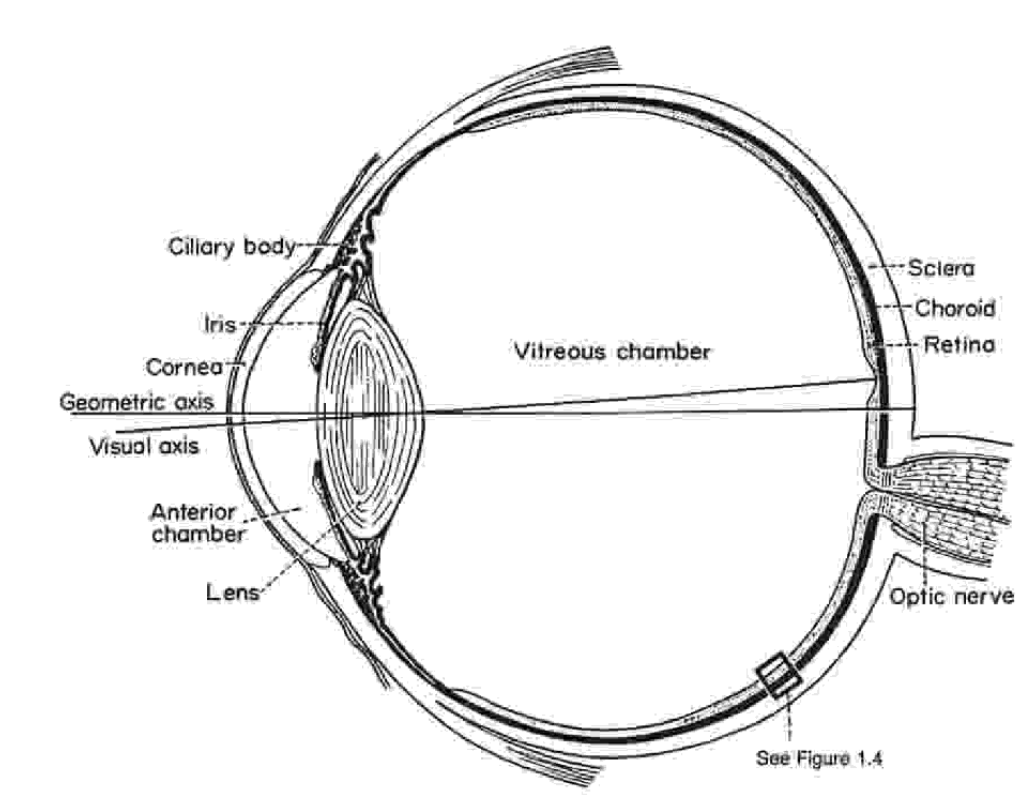
\includegraphics[width=\textwidth]{images/TheEye.png}
 \decoRule
 \caption[The Eye]{The Eye: Scientific drawing of the human eye, the organ responsible for the visual sense. Labels name the most important physiological structures, especially the lens that focuses light and the retina on which phototransduction takes place. Horizontal lines illustrate incident light rays hitting the retina. Taken from \protect\textcite{fatt2013physiology}}
 \label{fig:Eye}
\end{figure}

\subsection{Photo-receptors and Photo-transduction}
Photo-receptors consist of two parts. The inner segment is the cell body responsible for the general metabolism and the continuous construction of the outer segment. The outer segment is made up of membrane stacks which are permeated by Rhodopsin, a peptide composed of a trans-membrane domain and an attachment site for retinal. Retinal is a visual pigment that switches from 11-cis to all-trans configuration by the influence of a photon, thereby starting the phototransduction cascade, the initiation of the sensual process by creating a receptor potential. This signal is then transmitted via the synaptic terminal of the inner segment to the bipolar cells and then onto the ganglion cells. The axons of the bipolar cells form the optic nerve and therefore send signals to regions in the brain-stem \parencite{kolb1995webvision}. Importantly, the location of retinal cells is reflected in upstream areas, specifically in the optic nerve and later becomes prominent in the first visual cortex. This means that cells that are close together tend to send signals that are also processed in closely located areas in the upstream processing of the visual stimulations \parencite{selhorst2009optic}.


There are two types of photoreceptors that diverge in their shape and photoreception: Rods are thin, long and rod-shaped cells. They all contain the same visual pigment, which absorbs a wide range of wavelengths. Therefore, they are very efficient in collecting light, but they cannot distinguish between wavelengths. The perceptual outcome is black and white vision also in situations with low light exposure \parencite{kolb1995webvision}.

The cones are shorter and more cone-shaped. The outer segment does not contain as many membrane piles as rods. Thus, more light is necessary to elicit excitation of these cells. Cones are subdivided into three different types depending on the wavelength at which they maximally absorb. Short cones (S) absorb most efficiently short wavelengths which represents mostly blue and violet. Medium cones (M) absorb best in the green area, and long cones (L) are most sensitive to long wavelengths perceived as red. "S" cones are proportionally low in abundance, as the "M" and "L" cones occur around 100 times more often. But the overall relative composition of the different types is highly individual and might be the source of variation in color perception across humans. Namely, the brain uses the discrimination between wavelengths and the proportional excitation of these three types of receptor cells to process color vision \parencite{kolb1995webvision}.

In addition to the shape, cones and rods differ also in the region they occupy on the retina. The Fovea is almost exclusively populated with cones, while rods are placed in the periphery. Therefore, the Fovea is the place of color and the most precise vision. Low precision and non-chromatic vision of the peripheral regions are compensated for by constant scanning movements of the eye over the scenery and the brain's processing power, completing the mental image \parencite{kolb1995webvision}.


\subsection{Brain-stem}
The optical nerve leaving the eye is connected to the central nervous system. As a first step, the tracts cross in the Optic-Chiasm and through partial decussation information of both eyes coming from the right facial field is directed to the right hemisphere and vice versa. A smaller part of the nerve projects into the pretectal area, which is responsible for unconscious reflexes such as accommodation and pupillary reflex. Another subprojection aims for the superior colliculus which integrates somatosensory, auditory, and visual information in different layers forming, e.g. maps of the respective space. In "earlier" vertebrates this is the region of most complex processing and enables reflexes such as the intuitive focusing of newly approaching auditory or visual stimuli in the periphery. Furthermore, premotor areas code for movements towards specific areas in space. However, this region also integrates top down projections from the cortex which enables conscious intervention \parencite{fernandez2010anatomy, hubel1979BrainMech}.

The major part of the optical axons enter the Thalamus, more specifically, the corpus geniculatum laterale, which is considered to be the gatekeeper for all information entering the cortex and is constructed of six layers. These layers receive information from either the contra-lateral or ipsi-lateral side and are differentiated based on the ganglion cells from which they receive information. Layers one and two receive information from magnocellular ganglion cells, whereas layers 3 to 6 receive input from parvocellular ganglion cells. Magnocellular cells integrate over a broader number of sensory cells enabling the brain to process with higher speed and, therefore, support the perception of moving object in the visual scene. This is even exacerbated by heavily myelinated axons. The parvocellular ganglion cells integrate on fewer sensory cells, allowing for higher resolution and color perception \parencite{fernandez2010anatomy, hubel1979BrainMech}.

This differentiation represents the beginning of two hypothesized paths of visual processing that are supposed to be different in their objective: the "What" path and the "Where" path. The "What" path includes the precise identification of objects and their properties such as color or shape \parencite{grill2001lateral}. The "Where" path processes the rapid location of objects in space and their movement \parencite{gottlieb2007thought}. This separation is conserved in further processes in the cortex \parencite{ferrera1994responses, malach2002topography,mishkin1983object}.

\begin{figure}[htp]
 \centering
 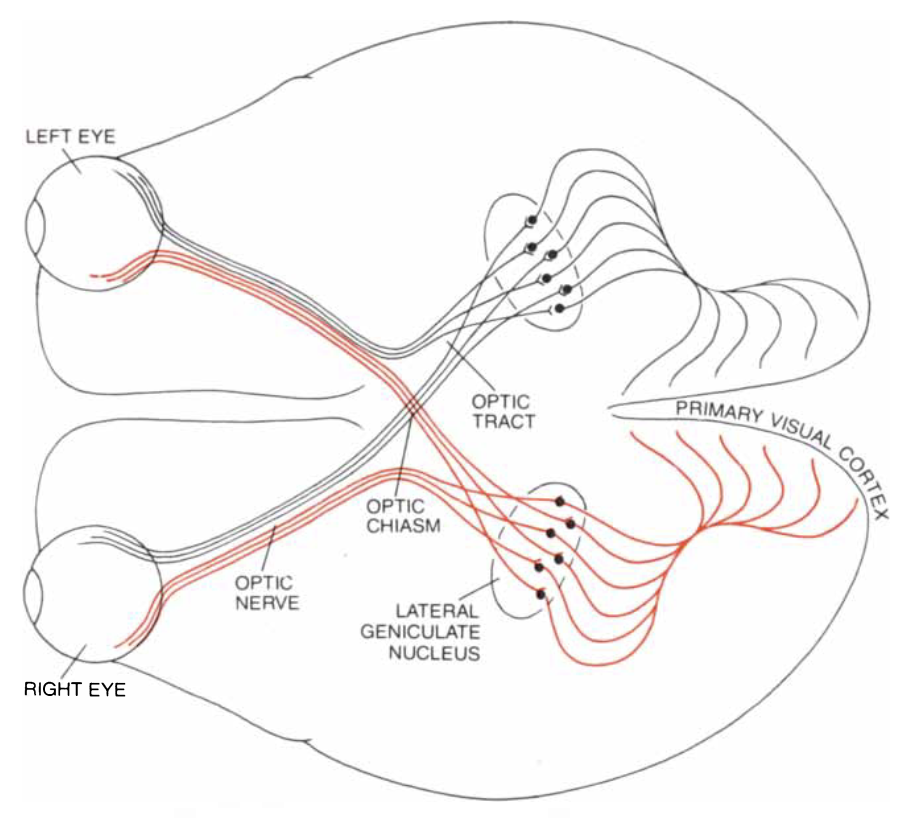
\includegraphics[width=\textwidth]{images/visual_pathway.png}
 \decoRule
 \caption[Visual Pathway]{Visual Pathway: The axons of the ganglion cells leave the retina and partially cross in the optic chiasm. Projections enter regions in the brain stem (pretectal area, Superior Colliculus, and the six layers of the lateral geniculate nucleus - thalamus). From there information is passed on to the primary visual cortex located in the occipital lobe.
 Taken from \protect\textcite{hubel1979BrainMech}}
 \label{fig:visual_pathway}
\end{figure}

\subsection{Visual Cortex}
Subsequently, the information is passed on to the fourth layer of the primary visual cortex, which is located in the occipital lobe. In the primary visual cortex, the retinotopic arrangement is conserved, which means that neighboring ganglion cells of the retina project to neighboring cells in the visual cortex. The overall organization is based on an the "ice-cube-model" \parencite{hubel1962receptive, hubel1979BrainMech}. Every point in the visual scene is represented by columns of neurons that respond to specific orientations of lines and edges. Additionally, there are so called blobs of neurons processing colors of the respective point in space \parencite{horton1984cytochrome, hubel1979BrainMech}. This implies that contours and colors in the visual scene are processed separately up until the second visual cortex. Once information leaves the visual cortex, it interacts with all other brain systems including memory, decision making and other executive functions \parencite{froudarakis2019Annual}. Ultimately, visual information contributes to actions. This hierarchy of processing is also a simplification. Naturally, sometime low level visual information is tightly integrated with actions and decision making. A simple example is a basketball player that needs to decide how to through a ball, coordinate visual information with its own motion and motor planning \parencite{pennartz2023howvisu}. 


From there, information is transmitted toward higher-order regions of the visual system. In the cortex visual processing is organized in different regions that are responsible for specific tasks of growing complexity, with "earlier" regions taking on more primitive tasks and higher-order areas such as the Inferior Temporal Lobe being engaged in complex tasks such as face recognition \parencite{sugase2011role}. The two previously mentioned paths can also be found here and determine the functions of the neighboring regions. Areas where an object's properties are studied are lined up around the temporal side of the cortex whereas regions that process motion are positioned toward the Paritetal Cortex \parencite{gegenfurtner1996interaction, niebur1995control}.


%\subsection{Higher order cortices and pathways}


